%%
%% This is file `sample-authordraft.tex',
%% generated with the docstrip utility.
%%
%% The original source files were:
%%
%% samples.dtx  (with options: `authordraft')
%% 
%% IMPORTANT NOTICE:
%% 
%% For the copyright see the source file.
%% 
%% Any modified versions of this file must be renamed
%% with new filenames distinct from sample-authordraft.tex.
%% 
%% For distribution of the original source see the terms
%% for copying and modification in the file samples.dtx.
%% 
%% This generated file may be distributed as long as the
%% original source files, as listed above, are part of the
%% same distribution. (The sources need not necessarily be
%% in the same archive or directory.)
%%
%% The first command in your LaTeX source must be the \documentclass command.
%\documentclass[sigconf,authordraft]{acmart}
\documentclass[sigconf, nonacm]{acmart}
\settopmatter{printacmref=false}
\renewcommand\footnotetextcopyrightpermission[1]{} 
\pagestyle{plain}
%% NOTE that a single column version may required for 
%% submission and peer review. This can be done by changing
%% the \doucmentclass[...]{acmart} in this template to 
%% \documentclass[manuscript,screen]{acmart}
%% 
%% To ensure 100% compatibility, please check the white list of
%% approved LaTeX packages to be used with the Master Article Template at
%% https://www.acm.org/publications/taps/whitelist-of-latex-packages 
%% before creating your document. The white list page provides 
%% information on how to submit additional LaTeX packages for 
%% review and adoption.
%% Fonts used in the template cannot be substituted; margin 
%% adjustments are not allowed.

%%
%% \BibTeX command to typeset BibTeX logo in the docs
\AtBeginDocument{%
  \providecommand\BibTeX{{%
    \normalfont B\kern-0.5em{\scshape i\kern-0.25em b}\kern-0.8em\TeX}}}

%% Rights management information.  This information is sent to you
%% when you complete the rights form.  These commands have SAMPLE
%% values in them; it is your responsibility as an author to replace
%% the commands and values with those provided to you when you
%% complete the rights form.
% \setcopyright{acmcopyright}
%% \setcopyright{acmcopyright}
% \copyrightyear{2021}
% \acmYear{2021}
%%  \acmDOI{10.1145/1122445.1122456}
% \acmDOI{}

%% These commands are for a PROCEEDINGS abstract or paper.
 \acmConference[Gatech CSE 8803-EPI]{Gatech CSE 8803-EPI final project}{August - December, 2021}{Atlanta, GA}
% \acmBooktitle{Woodstock '18: ACM Symposium on Neural Gaze Detection,
%   June 03--05, 2018, Woodstock, NY}
% \acmPrice{15.00}
% \acmISBN{978-1-4503-XXXX-X/18/06}


%%
%% Submission ID.
%% Use this when submitting an article to a sponsored event. You'll
%% receive a unique submission ID from the organizers
%% of the event, and this ID should be used as the parameter to this command.
%%\acmSubmissionID{123-A56-BU3}

%%
%% The majority of ACM publications use numbered citations and
%% references.  The command \citestyle{authoryear} switches to the
%% "author year" style.
%%
%% If you are preparing content for an event
%% sponsored by ACM SIGGRAPH, you must use the "author year" style of
%% citations and references.
%% Uncommenting
%% the next command will enable that style.
%%\citestyle{acmauthoryear}

%%
%% end of the preamble, start of the body of the document source.
\begin{document}
%%
%% The "title" command has an optional parameter,
%% allowing the author to define a "short title" to be used in page headers.
\title{Modeling the impact of vaccination, mask policies and mobility on the COVID-19 pandemic in Singapore}

%%
%% The "author" command and its associated commands are used to define
%% the authors and their affiliations.
%% Of note is the shared affiliation of the first two authors, and the
%% "authornote" and "authornotemark" commands
%% used to denote shared contribution to the research.

\author{Zishu Liu}
\email{zliu801@gatech.edu}
\authornote{All authors contributed equally to this research.}

\author{Yuxin Xie}
\email{yxie380@gatech.edu}
\authornotemark[1]

\author{Jichuan Zhang}
\email{jzhang3295@gatech.edu}
\authornotemark[1]

% \author{Ben Trovato}
% \email{trovato@corporation.com}
% \orcid{1234-5678-9012}
% \author{G.K.M. Tobin}
% \authornotemark[1]
% \email{webmaster@marysville-ohio.com}
% \affiliation{%
%   \institution{Institute for Clarity in Documentation}
%   \streetaddress{P.O. Box 1212}
%   \city{Dublin}
%   \state{Ohio}
%   \country{USA}
%   \postcode{43017-6221}
% }

% \author{Lars Th{\o}rv{\"a}ld}
% \affiliation{%
%   \institution{The Th{\o}rv{\"a}ld Group}
%   \streetaddress{1 Th{\o}rv{\"a}ld Circle}
%   \city{Hekla}
%   \country{Iceland}}
% \email{larst@affiliation.org}

% \author{Valerie B\'eranger}
% \affiliation{%
%   \institution{Inria Paris-Rocquencourt}
%   \city{Rocquencourt}
%   \country{France}
% }

% \author{Aparna Patel}
% \affiliation{%
%  \institution{Rajiv Gandhi University}
%  \streetaddress{Rono-Hills}
%  \city{Doimukh}
%  \state{Arunachal Pradesh}
%  \country{India}}

% \author{Huifen Chan}
% \affiliation{%
%   \institution{Tsinghua University}
%   \streetaddress{30 Shuangqing Rd}
%   \city{Haidian Qu}
%   \state{Beijing Shi}
%   \country{China}}

% \author{Charles Palmer}
% \affiliation{%
%   \institution{Palmer Research Laboratories}
%   \streetaddress{8600 Datapoint Drive}
%   \city{San Antonio}
%   \state{Texas}
%   \country{USA}
%   \postcode{78229}}
% \email{cpalmer@prl.com}

% \author{John Smith}
% \affiliation{%
%   \institution{The Th{\o}rv{\"a}ld Group}
%   \streetaddress{1 Th{\o}rv{\"a}ld Circle}
%   \city{Hekla}
%   \country{Iceland}}
% \email{jsmith@affiliation.org}

% \author{Julius P. Kumquat}
% \affiliation{%
%   \institution{The Kumquat Consortium}
%   \city{New York}
%   \country{USA}}
% \email{jpkumquat@consortium.net}

%%
%% The abstract is a short summary of the work to be presented in the
%% article.
\begin{abstract}
  In this project, we will use cutting-edge epidemiology models to study the impact of vaccination, mask policies and mobility on the outbreak of COVID-19 in Singapore.
\end{abstract}

%%
%% The code below is generated by the tool at http://dl.acm.org/ccs.cfm.
%% Please copy and paste the code instead of the example below.
%%
\begin{CCSXML}
<ccs2012>
   <concept>
       <concept_id>10010147.10010341.10010342.10010344</concept_id>
       <concept_desc>Computing methodologies~Model verification and validation</concept_desc>
       <concept_significance>500</concept_significance>
       </concept>
 </ccs2012>
\end{CCSXML}

\ccsdesc[500]{Computing methodologies~Model verification and validation}

%\ccsdesc[500]{Applied computing~Health informatics}

%%
%% Keywords. The author(s) should pick words that accurately describe
%% the work being presented. Separate the keywords with commas.
%\keywords{None}

%% A "teaser" image appears between the author and affiliation
%% information and the body of the document, and typically spans the
%% page.
% \begin{teaserfigure}
%   \includegraphics[width=\textwidth]{sampleteaser}
%   \caption{Seattle Mariners at Spring Training, 2010.}
%   \Description{Enjoying the baseball game from the third-base
%   seats. Ichiro Suzuki preparing to bat.}
%   \label{fig:teaser}
% \end{teaserfigure}

%%
%% This command processes the author and affiliation and title
%% information and builds the first part of the formatted document.
\maketitle

\section{Introduction}
The outbreak of a new crown outbreak depends on many factors, among which human influences include population mobility patterns, mask prevalence, and vaccination rates. The research in our project addresses the three important factors mentioned above. All three factors are influenced to some extent by government policies, and government decisions can be seen to influence the trend of the epidemic. We selected two outbreak trends in Singapore, which are listed below:
\begin{itemize}
	\item Singapore, March 2020 to Sept 2020 (optional)
	\item Singapore, July 2021 till now, mainly delta variant
\end{itemize}

There are significant differences among these two outbreaks. For example, during the last year's outbreak in Singapore, there were no available vaccines, but the government had published very strict policies to reduce social interactions. And for this year's outbreak in Singapore, nearly 90\% of people have been fully vaccinated, but the government is entering the `Preparatory Stage' and the local restrictions have been relaxed. The difference in vaccination rates and population mobility can help us to make a more accurate analysis of the impact of vaccination, mask policies and mobility. We hope that by studying these three factors and analyzing their weights on the outbreak trends, we can help the government to develop more effective prevention strategies to achieve successful protests. At the same time, we verify whether our research model is reasonable through data to achieve the purpose of accurately predicting the future trend of the epidemic.
\section{Response to the comments of our milestone report}
\begin{itemize}
	\item We add a title for the project.
	\item We add a SIR ODE model fitting the Singapore data to figure out the range of parameters and perform the calibration in a larger period with more parameters in this project. See the section \ref{sec-ode} for details.
	\item We use optuna to do the calibration in this project on first outbreak and second outbreak of Singapore separately in the period from last year to this years. Calibration details are discussed in section \ref{sec-cal}.

\end{itemize}
\section{Literature review}
We summarize and outline some information from papers related to agent models, including a new approach to predict the spread of COVID-19 in facilities based on agent models, the COVID-ABS agent model, the impact of the number of masks used globally on the outbreak discussed based on agent models, and the analysis of Australian data based on agent models. One of the emerging approaches based on agent models is used to represent complex systems comprising agents whose behavior is specified using simple rules \cite{cuevas2020agent}. This method differs from mathematical analyses of LGBT communities in that it represents individuals with a variety of characteristics, resulting in more realistic results. An agent-based strategy is offered for assessing COVID-19 transmission concerns in facilities. The spatio-temporal transmission mechanism is modeled in this way. Simulating spatio-temporal transmission mechanisms and simulating agents making judgments based on pre-programmed criteria are the foundations of this technology. These rules represent the geographical patterns and infectious situations with which the agents interact to explain the infection process. The model is extremely versatile, allowing for the testing of various hypotheses as well as alternative scenarios by considering hypothetical conditions that cannot be studied in real life. When compared to experimental methods, using this agent-based model offers the advantage of saving time and money. The ABS proxy model \cite{silva2020covid}, which simulates the epidemiological and economic impact of the COVID-19 pandemic in closed societies and whose results can be generalized in a broader context and used by government rulers to predict social policies and evaluate their effectiveness in real-world scenarios, is similar to this. This model creates novel situations by taking into account the unique characteristics of several research areas. The future study hopes to improve the model by incorporating methods for closing and opening organizations, as well as the ability to fire workers. Based on various scenarios as well as government planning, the model can potentially be optimized as a library. In another paper \cite{kai2020universal}, the movement of ABS agent models to predict the effect of masking on virus transmission is also mentioned in the literature. The paper compared two different pandemic viruses, including the recent COVID-19, based on this agent-based model, and the researchers compared the model's predictions with a large body of data to show a strong correlation between mask-wearing and the increase and decrease in daily cases. Fine-grained computational simulations \cite{chang2020modelling} of the pandemic were generated for Australia based on an agent model, and strategies to control for COVID-19 mitigation and suppression were introduced from the simulation data results, which were calibrated to match key features of COVID-19 transmission, with an important calibration result being the age-related scores of symptomatic cases. Above we have discussed and referred to some new technologies about the application of the proxy model and the impact of using this model on the trend of wearing masks on the pandemic and the prediction application based on Australian data and proxy models. These favorable information and analysis are useful for our project. Progress has helped a lot and brought us more ideas.
\section{Data source}
The data source for this study are listed below, which is also available at this \href{https://drive.google.com/drive/folders/1nVRsTTLyp0k4gV46zZ6d8C2gQEJnXjfd?usp=sharing}{link}. For a quick overview, Figure \ref{confirm} shows the daily confirmed COVID-19 cases/deaths and Google (residential) mobility trends of Singapore from February 17th 2020 to Oct 29th 2021.
\begin{itemize}
	\item COVID-19 cases/deaths/vaccines: The COVID-19 related data comes from \href{https://data.world/hxchua/covid-19-singapore}{data.world}. We choose several data points and verify it with \href{https://www.moh.gov.sg/covid-19/past-updates}{official MOH report}. For the missing vaccine data (from Jan 11th 2021 to June 30th 2021), we fill it with data from \href{https://ourworldindata.org/covid-vaccinations?country=SGP}{Our World in Data} and perform linear interpolation to make it continuous.
	\item Epidemiology: The epidemiology data of COVID-19, such as duration parameters (for example, duration between exposed state and infectious state), age-linked disease probability (for example, relative susceptibility to infection), is built in the library \href{https://github.com/InstituteforDiseaseModeling/covasim}{covasim}. 
	\item Demographics: The population age distribution data comes from this \href{https://github.com/neherlab/covid19_scenarios/blob/master/src/assets/data/ageDistribution.json}{Github repo} and is built in the library \href{https://github.com/InstituteforDiseaseModeling/covasim}{covasim}. However, because the Department of Statistics of Singapore only releases the resident population age distribution, we are not able to verify the correctness of this data.
	\item Mobility: We use \href{https://www.google.com/covid19/mobility/}{Google Community Mobility Reports} as the indicator of mobility. The reports provide the changes in movement trends across different categories of activities, which includes residential, retail and recreation, groceries and pharmacies, parks, transit stations, and workplaces. We collect this data from \href{https://ourworldindata.org/covid-google-mobility-trends}{Our World in Data}.
	\item Policy: We use \href{https://github.com/OxCGRT/covid-policy-tracker/tree/master/data}{mask policy indicator}, which is categorized into five categories: 0 - no policy; 1 - recommended; 2 - required in specified public spaces; 3 - required in all public spaces; 4 - required outside the home at all times. We also collect other relevant policy data (such as quarantine policy, face covering policy) from \href{https://www.moh.gov.sg/covid-19/past-updates}{official MOH report}.
\end{itemize}
\begin{figure}[htbp]
	\centering
	\includegraphics[width=0.9\linewidth]{data/confirmed.pdf}
	\caption{Daily COVID-19 counts and Google mobility trends}
	\label{confirm}
\end{figure}
\section{ODE Model}
\label{sec-ode}
In this section, we use the simple SIR ODE model to fit the COVID-19 data in Singapore as a supplement to our complicated agent-based model and to get a basic idea about the ranges of the parameters.
\subsection{Background and domain research}
First we plot the daily confirmed data before and after vaccination to have an intuitive understanding on the outbreaks of COVID-19 in Singapore (Figure \ref{sir0} and Figure \ref{sir1}).

\begin{figure}
	\centering
	\includegraphics[scale = 0.5]{Final/ode model/before-2.jpg}
	\caption{Daily Confirmed before vaccination}
	\label{sir0}
\end{figure}
\begin{figure}
	\centering
	\includegraphics[scale = 0.5]{Final/ode model/after.jpg}
	\caption{Daily Confirmed after vaccination}
	\label{sir1}
\end{figure}
As the daily confirmed infectious data shows, there are mainly three outbreaks: the first peaks around May 2020, and the second starts from September 2021.

The outbreak around May 2020 according to the news report and the statistics data provided by the Ministry of Health (MOH) Singapore , happens mainly among the foreign workers who live in the crowded dorms. The outbreak starts from September 2021 is caused by Singapore's new policy that treats COVID-19 in the way of treating flu, including opening the board and canceling the guarantee requirements for specific travelers, which loosens the intervention upon the COVID-19 to a great extent and causes a wide spread in communities.

The first outbreak and the second outbreak happened in different vaccination and policy backgrounds. Thus if we want to get the effectiveness of vaccination upon the outbreak, at least we need to integrate the effectiveness of policy into my ODE equations.




\subsection{Model Description}
Because all infectious cases, including asymptomatic infectious cases and cases in incubation periods are also counted to the confirmed cases and are required isolation, we remove the exposed states in SEIR model and use the SIR model instead.

There are four compartments in our ODE model, with the Infectious comprising two states - Hospitalized and Isolated. Below is the flow among the compartments (See Figure \ref{sir2} and the ODE equations).
\begin{figure}
	\centering
	\includegraphics[scale = 0.5]{Final/ode model/ode model.jpg}
	\caption{Flow Diagram of our SIR model}
	\label{sir2}
\end{figure}
\begin{equation}
\begin{cases} ds/dt = -\beta S(t) I(t) (1 + mobility(t)/100)/N \\ di/dt = \beta s I(t) (1 + mobility(t)/100)/N - \gamma I(t) - (I) r_d\\ dd/dt = I(t) r_d \\ dh/dt = di/dt \times r_h\\ dr/dt = \gamma I(t) \end{cases}
\end{equation}

The Singapore COVID-19 dataset we get includes the basic datas that are related to the COVID-19 contamination in a region and its policies to intervene in the COVID-19. However data likes the exact number of confirmed infectious cases and the number of the hospitalized people are not enough to directly measure  specific states in ODE model. And due to factors like testing policies and statistical granularity, there might be inaccurate or missing data. Thus we researched Singapore's COVID-19 policies and the statistical report provided by the MOH and found proper statistical data for S, I, R states.

For the S states, I first set S =  Population - I - R.

For the I states, we set I  = Intensive Care Unit (ICU) + General Wards + In Isolation. This is the way MOH uses to calculate the number of the active infectious cases. And thanks to Singapore's strict social lockdown and tracking spread policies, this data is accurate enough to reflect the infectious situation.

For the R states, we set R = Cumulative Confirmed - Cumulative Death - I.



\subsection{ Model fitting}

We use the minimize function in lmfit module (Non-Linear Least-Squares Minimization and Curve-Fitting), which implements the Levenberg-Marquardt algorithm to minimize the error between the measured data and the fitted data.
At the start, we set the error as below, where $m$ indicates measured and $f$ indicates fitted.

\begin{equation}
\begin{split}
    error =\sum_{t}\bigl\{&(St_{m} - St_{f})^2+(It_{m} - It_{f})^2\\
    &+(Rt_{m} - Rt_{f})^2 +(Dt_{m} - Dt_{f})^2\bigr\}^{1/2}
\end{split}
\end{equation}

The problem within such residual can include:
\begin{itemize}
    \item Trying to minimize the error for fitting three curves at the same time leads to failure in every single curve.
    \item The absolute error for different curve is quite different. The value of S is much bigger than the value of I and the value of R thus it should allow bigger absolute error.
\end{itemize}

Thus we changed my fitting method to fit only one curve for one iteration. First we fit the Infectious curve, and then the death curve and the recovery curve.

After one iteration of fitting, we found it's hard to fit the infectious curve because the rate of Suspicious almost remains unchanged due to the sparsity of infectious case and the strict social lockdown policy in Singapore. With the s / N remains approximately 1, di/dt = beta * i (1+ mobile[t]) - gamma * i - rd * i and whether di/dt > 0 or di/dt < 0  is only influenced by mobile[t] (The mobility data is shown in Figure \ref{sir3} and \ref{sir4}).
\begin{figure}
	\centering
	\includegraphics[scale = 0.5]{Final/ode model/mobility before.jpg}
	\caption{Mobility Before Vaccination}
	\label{sir3}
\end{figure}
\begin{figure}
	\centering
	\includegraphics[scale = 0.5]{Final/ode model/mobility after.jpg}
	\caption{Mobility After Vaccination}
	\label{sir4}
\end{figure}

So after reading some papers who fit SEIR and SIR model to the real dataset, we decide to narrow the clique of COVID-19 spread in Singapore and set the total number of people rather than the population of Singapore, but instead as 110000 who are possible to engage in the spread and the number of the susceptible as 90000, and get a good fit.

\subsection{Observations}
As the fit results indicate, the beta of the first outbreak (May 2020) is 0.44964359, while the beta of the second outbreak (September 2021) is 0.18322612. With a more loose overall policy, the second outbreak still gain a better beta, which indicates that the vaccine has effectively prevented the spread of COVID-19.








\section{Agent-based Model}
In this section, we provide a formal description of \href{https://github.com/InstituteforDiseaseModeling/covasim}{covasim} model \citep{kerr2021covasim} and how we model vaccinations, mask policies and mobility changes within our model.
\subsection{Disease progression}
\begin{figure}
	\centering
	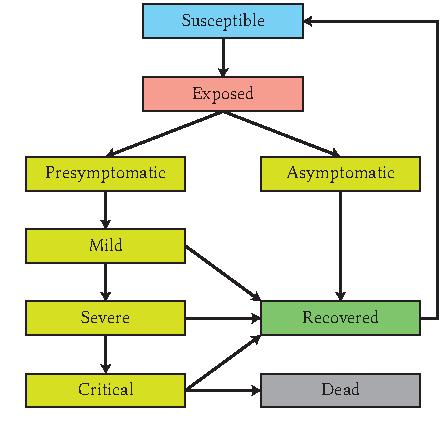
\includegraphics{model/seir.pdf}
	\caption{Covasim model, disease state transformation structure}
	\label{seir}
\end{figure}

In covasim, the disease state of an agent is characterized as susceptible, exposed, infectious (asymptomatic, presymptomatic, mild, severe, critical), recovered and dead. The Figure \ref{seir} shows all possible transformation between any two disease states. Each transformation is also parameterized with a probability $p$ (how likely does the transformation happen) and a duration $\tau$ (how long does the transformation take). The age-linked value of $p$ and the distribution of $\tau$ are detrived from lots of previous research and are built in \href{https://github.com/InstituteforDiseaseModeling/covasim}{covasim}.

\subsection{Contact network}

To model the contact network between people, covasim assigns people to four network layers: household, school, workplace and community. More specifically, covasim generates a population of people based on the location-specific age distribution. After that, covasim assigns people aged between 6 and 22 to schools, assigns people aged between 22 and 65 to workplaces and assigns people to households based on the location-specific household size.

Within each network, the contact number of each person is sampled from poisson distributions. For each contact between a susceptible individual and an infectious individual, the probability of a successful virus transmission is $\beta$.

\subsection{Agent states}

One important feature of covasim is that it provides several useful agent states so that it can describe testing, contact-tracing, quarantine and isolation policies. Figure \ref{state} lists out built in agent states and transformations between them.
\begin{itemize}
	\item Free: If an agent is free, the agent has $100\%~\beta$ value. If a free agent has a contact with a confirmed case and is traced successfully, the agent will become quarantined. If a free agent has positive test results, the agent will become isolated.
	\item Quarantined: If an agent is quarantined, the agent has $60\%~\beta$ in the household layer and $20\%~\beta$ in other layers. The quarantine ends when it reaches the maximum quarantine time. However, if a quarantined agent has positive test results, the agent will also get isolated.
	\item Isolated: If an agent is isolated, the agent has $30\%~\beta$ in the household layer and $10\%~\beta$ in other layers. A isolated agent will become free once the agent recovers.
\end{itemize}

\begin{figure}
	\centering
	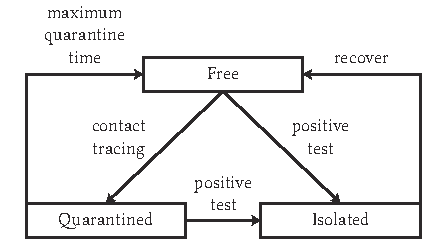
\includegraphics{model/state.pdf}
	\caption{Covasim model, agent state transformation structure}
	\label{state}
\end{figure}

\subsection{Mask policies and mobility}
There are two important factors which affect the spread of COVID-19. The first one is personal protection, such as wearing masks, washing hands, etc, which reduces the probability of virus transmission per contact, i.e., the $\beta$ value The second one is social distancing, such as avoiding crowds, keeping distance from others, staying at home, etc, which reduces the contact number of each agent.

Within our model, we use mask policies and mobility to represent personal protection and social distancing respectively. More specifically, denote numerical mask policies and mobility as $x_{\text{ma}},x_{\text{mo}}$, we define a function $f:\mathcal{R}^2\rightarrow[0,1]$ as:
\begin{equation}
	f(x_{\text{ma}},x_{\text{mo}})=\frac{2(a_1x_{\text{ma}}+b_1)(a_2x_{\text{mo}}+b_2)}{(a_1x_{\text{ma}}+b_1)+(a_2x_{\text{mo}}+b_2)}
\end{equation}

We can view this function as first applying two linear transformation on $x_1=a_1x_{\text{ma}}+b_1$, $x_2=a_2x_{\text{mo}}+b_2$ and then apply the function $g(x_1,x_2)=2x_1x_2/(x_1+x_2)$. We can view the function $g$ in another way:

\begin{equation}
    \begin{split}
         g&(x_1,x_2)=\frac{2x_1x_2}{x_1+x_2}\\
         &=\min\{x_1,x_2\}\frac{\max\{x_1,x_2\}}{x_1+x_2} + \max\{x_1,x_2\}\frac{\min\{x_1,x_2\}}{x_1+x_2}
    \end{split}
\end{equation}

We design such function because we believe that the smaller value of $x_1,x_2$ has a larger impact of $\beta$. After that, for each day we calculate the $\beta$ value as $f(x_{\text{ma}},x_{\text{mo}})\beta_0$, where the $\beta_0$ is a constant within one outbreak (for a variant of SARS-CoV-2) and $x_{\text{ma}},x_{\text{mo}}$ changes each day.

\section{Agent-based model Results}
\label{sec-cal}
\subsection{Calibration process}
We use optuna to perform the calibration. Each time, we sample parameters from the Tree-structured Parzen Estimator (TPE) sampler and run the simulation once. After that, we calculate the minimization objective value as the mean absolute error of the cumulative confirmed number between the simulation results and the real-world data and feed the  objective value to sampler. Because of the limitation of hardware and time, we times all the cases/deaths/vaccines with 0.01. We use the negative of mask policy indicator and the negative of residential mobility as the numerical mask policies and mobility value. We model the first outbreak (from March 2020 to Sept 2020) and the second outbreak (from July 2021 to Oct 25th) separately because they are caused by different variants.

For the first outbreak, we calibrate the following parameters:

\begin{itemize}
	\item $\beta_0$: the probability of a successful virus transmission per contact, calibration range is $[0.06,0.10]$.
	\item $\text{ma}_{\min}$: we calculate $a_1$ and $b_1$ such that $\max\{a_1x_{\text{ma}}+b_1)\}=1.0$ and $\min\{a_1x_{\text{ma}}+b_1)\}=\text{ma}_{\min}$. The calibration range is $[0.03, 0.25]$.
	\item $\text{mo}_{\min}$: we calculate $a_2$ and $b_2$ such that $\max\{a_2x_{\text{mo}}+b_2)\}=1.0$ and $\min\{a_2x_{\text{mo}}+b_2)\}=\text{mo}_{\min}$. The calibration range is $[0.1, 0.6]$.
	\item $\text{symp\_prob}$: the test probability of a symptomatic agent, calibration range is $[0.9,1.0]$.
	\item $\text{trace\_probs}$: the successful probability of a contact tracing, calibration range is $[0.75,0.99]$.
	\item $\text{start\_shift}$: the number of days between the first ten people get infected and the first confirmed case, calibration range is $[-8,8]$.
\end{itemize}

Besides these parameters, we set the following parameters as constants:
\begin{itemize}
	\item $\text{pop\_infected}=10$: the number of infected people at the start of the simulation
	\item $\text{asymp\_prob}=0$: the test probability of a asymptomatic agent
	\item $\text{quar\_period}=7$: the maximum quarantine time in days, we collect the value from the official \href{https://www.covid.gov.sg/exposed/hrw}{MOH website}
	\item $\text{test\_delay}=1$: the number of days for test results to be known
\end{itemize}

After calibrating the first outbreak, we setup the second outbreak with the same constants and the calibration results $\text{ma}_{\min}$, $\text{mo}_{\min}$, $\text{symp\_prob}$, $\text{trace\_probs}$ of the first outbreak. For the second outbreak, we only calibrate the $\beta_0$ value in range $[0.61,0.3]$ and the $\text{start\_shift}$ in range $[-21,21]$ while take the vaccinations into consideration. Instead of introducing infected populations at the start of the simulation, we introduce 10 people infected by delta variant on the day when the first case gets confirmed (24th August) shifted by  $\text{start\_shift}$.

Regards the vaccination, we assume that people only receive Pfizer COVID-19 vaccines and the order in which people get vaccinated is the descending order of people's age. We also assume that people who have received the first dose 21 days before have priority in receiving the second dose. We calibrate the first outbreak with 5000 samples and the second outbreak with 2000 samples.

After calibrating the second outbreak, we assume the daily vaccine doses, mask policies and mobility as the mean of the last 30 days and predict the epidemiology data of the next 30 days, which lies in the yellow area of Figure \ref{cal2}.
\subsection{Calibration results}
\begin{figure}[htbp]
	\centering
	\includegraphics[width=0.95\linewidth]{result/sg_calib1_result.pdf}
	\caption{First outbreak, calibration results}
	\label{cal1}
\end{figure}
\begin{figure}
	\centering
	\includegraphics[width=0.95\linewidth]{result/sg_calib2_predict.pdf}
	\caption{Second outbreak, calibration results}
	\label{cal2}
\end{figure}
For the first outbreak, the calibrated parameters are $\beta_0=0.061$, $\text{ma}_{\min}=0.13$, $\text{mo}_{\min}=0.43$, $\text{symp\_prob}=0.9$, $\text{trace\_prob}=0.79$, $\text{start\_shift}=3$. Figure \ref{cal1} shows the calibration results of the first outbreak. The calibration results fit the data pretty well except the first month, which may results from the relatively low testing probability at the beginning.

For the second outbreak, the calibrated parameters are $\beta_0=0.134$, $\text{start\_shift}=10$. Figure \ref{cal2} shows the calibration results of the first outbreak and the prediction of the next 30 days (in yellow area). The calibration results not only fit the data well but also give a pretty good prediction. Cause the $\beta_0$ value has already been multiplied by 2.2 within covasim, the real $\beta_0$ value is $2.2\times 0.134\approx0.295$, which is about four times larger than the $\beta_0$ value of the first outbreak.
\subsection{Effect of vaccination}
\begin{figure}
	\centering
	\includegraphics[width=0.95\linewidth]{result/sg2_zero_predict.pdf}
	\caption{Second outbreak, without vaccination}
	\label{without}
\end{figure}
To evaluate the effect of the vaccination, we run the simulation of the second outbreak with same parameters but without vaccination. Figure \ref{without} indicates that more than a half of the total population will get infected under such mask policies and mobility, which reveals the importance of the vaccination.
\subsection{Effect of mask policies and mobility}
\begin{figure}
	\centering
	\includegraphics[width=0.95\linewidth]{result/sg_calib1_change.pdf}
	\caption{The impact of mask policies and mobility}
	\label{change}
\end{figure}
Figure \ref{change} shows the impact of mask policies and mobility on the $\beta$ value. When the mask policies are not strict, the change of mobility explains the main part of the change of $\beta$. However, when the mask policies becomes strict after mid-April, the change of mobility only causes small fluctuations on $\beta$.

\section{Conclusion and Discussion}

\subsection{ODE model}
The fitting method still needs improvement. For the fitting iterations, we only involve infectious data in residual function and minimize the error in fitting the infectious data to get an initial beta. Then we use the beta for following iterations for minimizing the error in fitting the death data and then the hospitalized data and then the recovery data. The beta doesn't change much during the iterations. For example, for the after vaccine outbreak, the beta after each iteration is : 0.18322830 -> 0.14602370 ->  0.20936286 -> 0.26362917. Though the beta doesn't change much during these iterations, every iteration fits the assigned curve well but doesn't perform as well in other curves (see Figure \ref{sir5}). So it is still not scientific enough to fit for only one parameter and one curve for one iteration. It would be better if all the curves are fitted at the same time in every iteration.
\begin{figure}
	\centering
	\includegraphics[scale = 0.5]{Final/ode model/after fit all-2.jpg}
	\caption{Fitting Results of the Second Outbreak}
	\label{sir5}
\end{figure}

Another point for improvement is to find a scientific way to measure and estimate the number of susceptible cases in real life spread. We get a good fit result by manually assigning the number of initial susceptible cases and we also see other researchers who set the number of initial susceptible cases as a value suggested by domain experts. So it would be very helpful for using the SIR and SEIR ODE model to research on real life problems if there is a more systematic and scientific method to get the number of S state cases in real life.

\subsection{Agent-based model}
The results of the agent-based model reveal the importance of vaccination and strict mask policies. Even the delta variant is highly infectious, with vaccination and strict mask policies the number of infections is still able to be controlled small. The mobility takes an important role when mask policies are relatively loose but contributes little to the spread of COVID-19 when mask policies are strict. Therefore, we strongly suggest that high vaccination rate and strict mask policies are vital for fighting against COVID-19.

However, there are several aspects that may be improved in the future research.

First, we assume that lots of parameters are constant within out model, such as test probability, contact tracing probability, quarantine period, etc. However, these parameters changes during the pandemic and highly depends on the government policies and the pandemic situation. Future research can focus on how the model the change of these parameters so that the model can represent the reality better.

What's more, covasim calculates the waning effect of vaccines based on the decreasing of neutralizing antibody \cite{khoury2021level} and calculates the effectiveness against the delta variant based on this paper \cite{mlcochova2021sars}. Because of limited time and knowledge, we are not able to verify the correctness of these values and models. The waning effect of vaccines and the effectiveness against different variants are hot topics in this area. We should also notice that Singapore has started the vaccine booster program from October 1st while the impact of the booster is still under research. Therefore, future research may be able to model the effectiveness of vaccines in a more accurate way.
\section{Appendix}
Code and datasets for this project are available at this \href{https://github.com/zs-liu/CSE8803-Singapore}{Github repo}.

\bibliographystyle{ACM-Reference-Format}
\bibliography{final.bib}
\end{document}
\endinput
%%
%% End of file `sample-authordraft.tex'.
